\section{Datapath}
\label{sec:datapath}

Darkriscv was simple in terms of the file hierarchy, but its internal structure
was not so trivial. For the reason of understanding the code accordingly and
preparing it for the next step--explained in section~\ref{sec:referee}--. We decided to
separate the different functionalities of the core into distinct modules.

\subsection{Modules}

Creating four modules in total; the program counter (PC), the fetch (or
instruction memory controller), the ALU/BR (for Arithmetic Logic Unit and
Register Bank) and the memory (or data memory controller). These modules will
expect their inputs to be stable and valid when its \textit{en} (abbreviation of
enable) signal is set to high--for one cycle--and until it sets its \textit{valid}
signal high--for one cycle--. The module will hold its output signals until the
enable is set high again.

\tikzset{every picture/.style={line width=0.75pt}} %set default line width to 0.75pt        

\begin{figure}[H]
  
  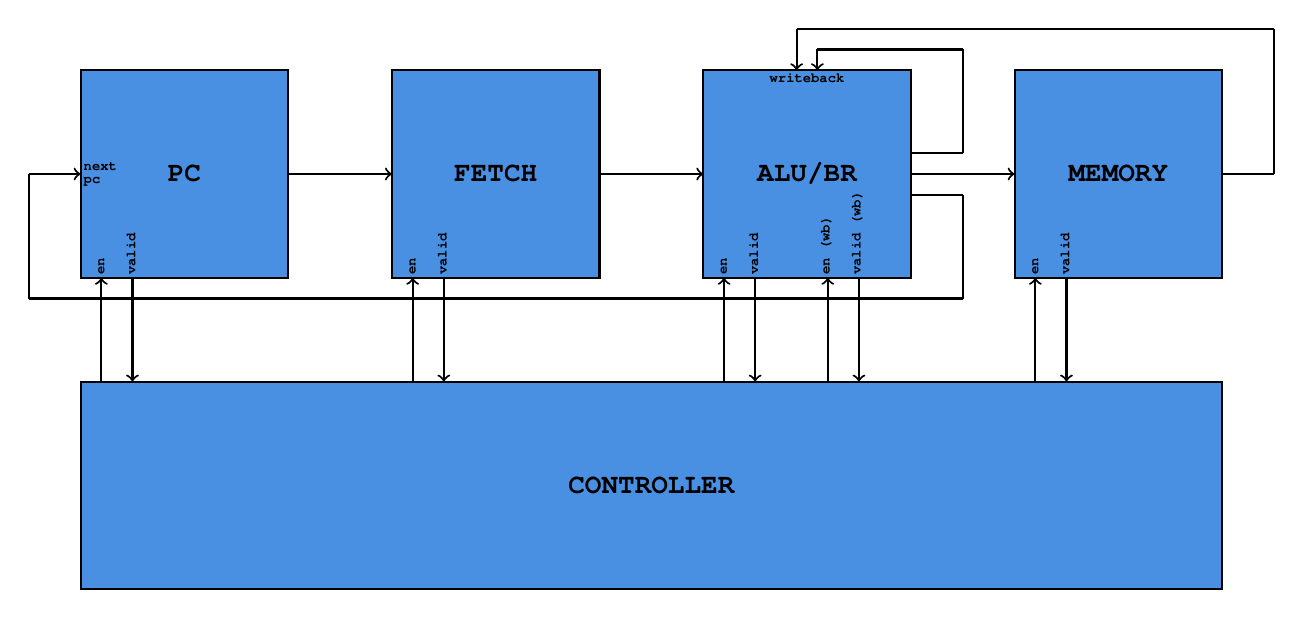
\begin{tikzpicture}[x=0.75pt, y=0.75pt, yscale=-1,xscale=1]
      
    \draw [fill={rgb, 255:red,  74; green, 144; blue, 226 }  ,fill opacity=1 ]
          (  0, 0) rectangle (100, 100)
          node [midway] {\fontfamily{pcr}\selectfont \textbf{PC}};

    \draw [fill={rgb, 255:red,  74; green, 144; blue, 226 }  ,fill opacity=1 ]
          ( 150, 0) rectangle (250, 100)
          node [midway] {\fontfamily{pcr}\selectfont \textbf{FETCH}};

    \draw [fill={rgb, 255:red,  74; green, 144; blue, 226 }  ,fill opacity=1 ]
          (300, 0) rectangle (400, 100)
          node [midway] {\fontfamily{pcr}\selectfont \textbf{ALU/BR}};

    \draw [fill={rgb, 255:red,  74; green, 144; blue, 226 }  ,fill opacity=1 ]
          (450, 0) rectangle (550, 100)
          node [midway] {\fontfamily{pcr}\selectfont \textbf{MEMORY}};

    \draw [fill={rgb, 255:red,  74; green, 144; blue, 226 }  ,fill opacity=1 ]
          (  0, 150) rectangle (550,250)
          node [midway] {\fontfamily{pcr}\selectfont \textbf{CONTROLLER}};


    % Line PC - FE
    \draw [->] (100,50) -- (150,50); %(100, 50) to (100, 50);

    % Line FE - Core
    \draw [->] (250,50) -- (300,50); %(100, 50) to (100, 50);

    % Line Core - ME
    \draw [->] (400,50) -- (450,50); %(100, 50) to (100, 50);

    % Line WB - Core
    \draw [-]  (400,40) -- (425,40); 
    \draw [-]  (425,40) -- (425,-10);
    \draw [-]  (425,-10) -- (355,-10);
    \draw [->] (355,-10) -- (355,0);

    % Memory - WB
    \draw [-]  (550,50) -- (575,50); 
    \draw [-]  (575,50) -- (575,-20);
    \draw [-]  (575,-20) -- (345,-20);
    \draw [->] (345,-20) -- (345,0);

    % Line Core - PC
    \draw [-]  (400, 60) -- (425, 60); 
    \draw [-]  (425, 60) -- (425,110);
    \draw [-]  (425,110) -- (-25,110);
    \draw [-]  (-25,110) -- (-25, 50);
    \draw [->] (-25, 50) -- (  0, 50);

    % Label: next pc
    \draw (350, 0) node [below][inner sep=0.75pt] {\tiny\fontfamily{pcr}\selectfont \textbf{writeback}};

    % Label: WB
    \draw (0, 50) node  [anchor=south west][inner sep=0.75pt] {\tiny\fontfamily{pcr}\selectfont \textbf{next}};
    \draw (0, 50) node  [anchor=north west][inner sep=0.75pt] {\tiny\fontfamily{pcr}\selectfont \textbf{pc}};

    % Labels: en/valid
    \draw (13,100) node [rotate=90,anchor=south west][inner sep=0.75pt] {\tiny\fontfamily{pcr}\selectfont \textbf{en}};
    \draw (28,100) node [rotate=90,anchor=south west][inner sep=0.75pt] {\tiny\fontfamily{pcr}\selectfont \textbf{valid}};
    \draw [<-] (10,100) -- (10,150);
    \draw [->] (25,100) -- (25,150);

    \draw (163,100) node [rotate=90,anchor=south west][inner sep=0.75pt] {\tiny\fontfamily{pcr}\selectfont \textbf{en}};
    \draw (178,100) node [rotate=90,anchor=south west][inner sep=0.75pt] {\tiny\fontfamily{pcr}\selectfont \textbf{valid}};
    \draw [<-] (160,100) -- (160,150);
    \draw [->] (175,100) -- (175,150);

    \draw (313,100) node [rotate=90,anchor=south west][inner sep=0.75pt] {\tiny\fontfamily{pcr}\selectfont \textbf{en}};
    \draw (328,100) node [rotate=90,anchor=south west][inner sep=0.75pt] {\tiny\fontfamily{pcr}\selectfont \textbf{valid}};
    \draw [<-] (310,100) -- (310,150);
    \draw [->] (325,100) -- (325,150);

    \draw (363,100) node [rotate=90,anchor=south west][inner sep=0.75pt] {\tiny\fontfamily{pcr}\selectfont \textbf{en (wb)}};
    \draw (378,100) node [rotate=90,anchor=south west][inner sep=0.75pt] {\tiny\fontfamily{pcr}\selectfont \textbf{valid (wb)}};
    \draw [<-] (360,100) -- (360,150);
    \draw [->] (375,100) -- (375,150);

    \draw (463,100) node [rotate=90,anchor=south west][inner sep=0.75pt] {\tiny\fontfamily{pcr}\selectfont \textbf{en}};
    \draw (478,100) node [rotate=90,anchor=south west][inner sep=0.75pt] {\tiny\fontfamily{pcr}\selectfont \textbf{valid}};
    \draw [<-] (460,100) -- (460,150);
    \draw [->] (475,100) -- (475,150);

  \end{tikzpicture}

  \caption{Datapath structure}
  \label{fig:datapath_mods}
\end{figure}

All the \textit{en} signals are managed by the datapath, which uses five stages.
Each stage only uses one module. The datapath will choose to go to the next
stage once the current module in use sets \textit{valid} to high. The ALU/BR module has
double functionality and is used in two separate stages. Firstly in the
processing (ALU) of all the data of the current instruction. And finally on the
writeback, where all the necessary data is written back to the register file (BR).

In figure \ref{fig:datapath_mods} we can see the diagram that represents the explained modules and
their data flow with the controller management.

\subsection{Memory managment}

Furthermore, we had to implement a memory bus selector
in order to multiplex between the two modules that make memory access. This
logic is controlled by the datapath--ass in figure~\ref{fig:datapath_mem}--.
Its implementation is easy the selector chooses the fetch module based on the
datapath stage. And disables the bus when neither the fetch nor the memory
stage is being executed.

\tikzset{every picture/.style={line width=0.75pt}} %set default line width to 0.75pt        

\begin{figure}[H]
  \centering
  
  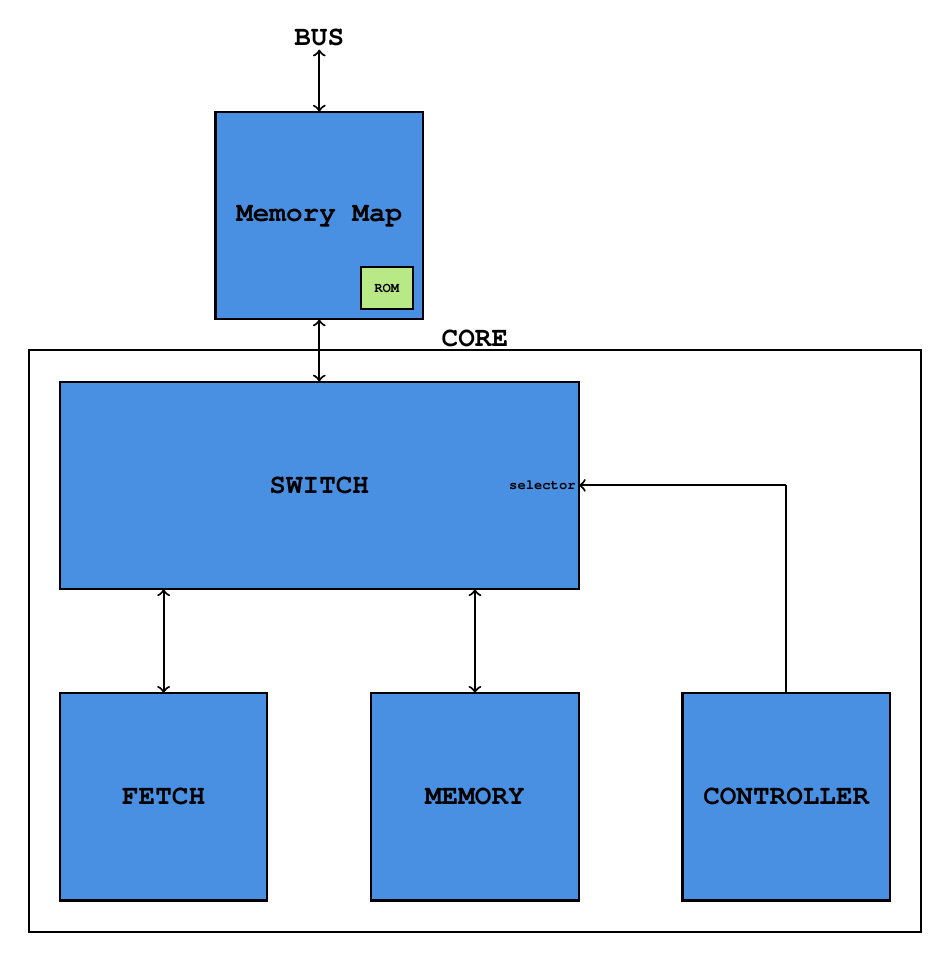
\begin{tikzpicture}[x=0.75pt, y=0.75pt, yscale=-1,xscale=1]

    \draw (200,-15) node [anchor=south,align=center][inner sep=0.75pt] {\fontfamily{pcr}\selectfont \textbf{CORE}};
    \draw [fill={rgb, 255:red,  74; green, 144; blue, 226 }  ,fill opacity=0 ]
          (-15,-15) rectangle (415,265)
          node [midway] {\fontfamily{pcr}\selectfont \textbf{}};

    \draw [fill={rgb, 255:red,  74; green, 144; blue, 226 }  ,fill opacity=1 ]
          (  0, 0) rectangle (250, 100)
          node [midway] {\fontfamily{pcr}\selectfont \textbf{SWITCH}};
      
    \draw [fill={rgb, 255:red,  74; green, 144; blue, 226 }  ,fill opacity=1 ]
          (  0, 150) rectangle (100, 250)
          node [midway] {\fontfamily{pcr}\selectfont \textbf{FETCH}};

    \draw [fill={rgb, 255:red,  74; green, 144; blue, 226 }  ,fill opacity=1 ]
          (150, 150) rectangle (250, 250)
          node [midway] {\fontfamily{pcr}\selectfont \textbf{MEMORY}};

    \draw [fill={rgb, 255:red,  74; green, 144; blue, 226 }  ,fill opacity=1 ]
          (300, 150) rectangle (400, 250)
          node [midway] {\fontfamily{pcr}\selectfont \textbf{CONTROLLER}};

    \draw [fill={rgb, 255:red,  74; green, 144; blue, 226 }  ,fill opacity=1 ]
          (75,-130) rectangle (175, -30)
          node [midway] {\fontfamily{pcr}\selectfont \textbf{Memory Map}};

    \draw [fill={rgb, 255:red, 184; green, 233; blue, 134 }  ,fill opacity=1 ] 
          (145,-55) rectangle (170, -35)
          node [midway] {\tiny\fontfamily{pcr}\selectfont \textbf{ROM}};

    \draw [<->] (125,   0) -- (125,-30); 
    \draw [<->] (125,-130) -- (125,-160); 
    \draw (125, -160) node [anchor=south,align=center][inner sep=0.75pt] {\fontfamily{pcr}\selectfont \textbf{BUS}};

    \draw [<->] ( 50, 100) -- ( 50,150); 
    \draw [<->] (200, 100) -- (200,150); 

    \draw [-]  (350,150) -- (350,50); 
    \draw [->] (350, 50) -- (250,50);

    \draw (250, 50) node [anchor=east][inner sep=0.75pt] {\tiny\fontfamily{pcr}\selectfont \textbf{selector}};

  \end{tikzpicture}

  \caption{Datapath bus switching}
  \label{fig:datapath_mem}

\end{figure}

Once the memory is out of the core the bus is intercepted by the memory mapper,
this module will manage, depending on the access address, the device that
should receive the petition. As shown in the figure~\ref{fig:memory_map} de
first 512 MiB are assign to the ROM holding the code. The ROM is inside the module itself
and is replicated for every core. Whereas, on the other hand, the last 3 GiB
are assigned to the RAM, which is an external device\footnote{In this case external 
device means that it is outside the core and memory map modules, but not external
to the FPGA.}.

It is important to mention that although the processor is able to execute code
from RAM it is not optimized for that.

\tikzset{every picture/.style={line width=0.75pt}} %set default line width to 0.75pt        

\begin{figure}
  \centering
  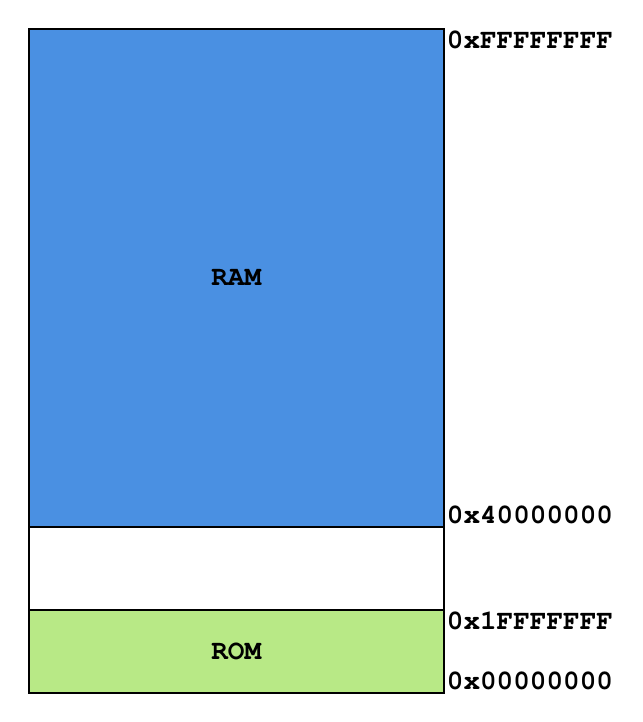
\begin{tikzpicture}[x=0.75pt,y=0.75pt,yscale=-1,xscale=1]
    %uncomment if require: \path (0,452); %set diagram left start at 0, and has height of 452

    %Shape: Rectangle RAM
    \draw [fill={rgb, 255:red,  74; green, 144; blue, 226 }  ,fill opacity=1 ] 
          (  0,   0) rectangle (200, 240) 
          node [midway] {\fontfamily{pcr}\selectfont \textbf{RAM}};

    %Shape: Rectangle void
    \draw [fill={rgb, 255:red, 255; green, 255; blue, 255 }  ,fill opacity=1 ] 
          (  0, 240) rectangle (200, 280) 
          node [midway] {};

    %Shape: Rectangle ROM
    \draw [fill={rgb, 255:red, 184; green, 233; blue, 134 }  ,fill opacity=1 ] 
          (  0, 280) rectangle (200, 320) 
          node [midway] {\fontfamily{pcr}\selectfont \textbf{ROM}};

    %Text: RAM addres range
    \draw (200,   0) node [anchor=north west][inner sep=0.75pt] {\fontfamily{pcr}\selectfont \textbf{0xFFFFFFFF}} ;
    \draw (200, 240) node [anchor=south west][inner sep=0.75pt] {\fontfamily{pcr}\selectfont \textbf{0x40000000}} ;

    %Text: Void addres range
    %\draw (200, 240) node [anchor=north west][inner sep=0.75pt] {\fontfamily{pcr}\selectfont \textbf{0x3FFFFFFF}} ;
    %\draw (200, 280) node [anchor=south west][inner sep=0.75pt] {\fontfamily{pcr}\selectfont \textbf{0x20000000}} ;

    %Text: ROM addres range
    \draw (200, 280) node [anchor=north west][inner sep=0.75pt] {\fontfamily{pcr}\selectfont \textbf{0x1FFFFFFF}} ;
    \draw (200, 320) node [anchor=south west][inner sep=0.75pt] {\fontfamily{pcr}\selectfont \textbf{0x00000000}} ;
  \end{tikzpicture}

  \caption{Memory mapping}
  \label{fig:memory_map}

\end{figure}


